\documentclass[11pt,a4paper]{article}

% ---------- Packages ----------
\usepackage[utf8]{inputenc}
\usepackage[T1]{fontenc}
\usepackage{lmodern}
\usepackage{amsmath,amssymb}
\usepackage{enumitem}
\usepackage{geometry}
\usepackage{fancyhdr}
\usepackage[most]{tcolorbox}   % enhanced, breakable
\usepackage{hyperref}
\usepackage[siunitx]{circuitikz}

% ---------- Geometry ----------
\geometry{margin=2.5cm}

% ---------- Header/Footer ----------
\setlength{\headheight}{14pt}  % fancyhdr warning verhindern
\pagestyle{fancy}
\fancyhf{}
\lhead{Einführung in die Elektrotechnik}
\rhead{Wintersemester 2025}
\cfoot{\thepage}

% ---------- Exercise Environment ----------
\newcounter{exercise}
\newenvironment{exercise}[1][]
  {\refstepcounter{exercise}%
   \begin{tcolorbox}[enhanced, breakable, width=\textwidth,
     colback=blue!5!white,colframe=blue!60!black,
     fonttitle=\bfseries\large,
     title=Aufgabe~\theexercise:~#1]}
  {\end{tcolorbox}}

% ---------- Solution Environment ----------
\newif\ifshowsolutions
\showsolutionstrue  % comment to hide solutions

\newenvironment{solution}
  {\ifshowsolutions
     \begin{tcolorbox}[enhanced, breakable, width=\textwidth,
       colback=green!5!white,colframe=green!50!black,
       fonttitle=\bfseries\large,
       title=Lösung]}
  {\end{tcolorbox}\fi}

% ---------- Document ----------
\begin{document}

% ----- Header Box -----
\begin{tcolorbox}[enhanced, breakable, colback=gray!10!white,
  colframe=gray!70!black, fonttitle=\bfseries\large,
  title={Aufgabenblatt \#2}: DC 1: Schaltungsberechnungen, sharp corners, width=\textwidth]
\begin{center}
  Besprechung: 22.10.2025
\end{center}
\end{tcolorbox}
\vspace{1cm}

% ----- Exercise 1 -----
\begin{exercise}[Topologie]
Bestimme die Anzahl der Knoten, Zweige und Schleifen.

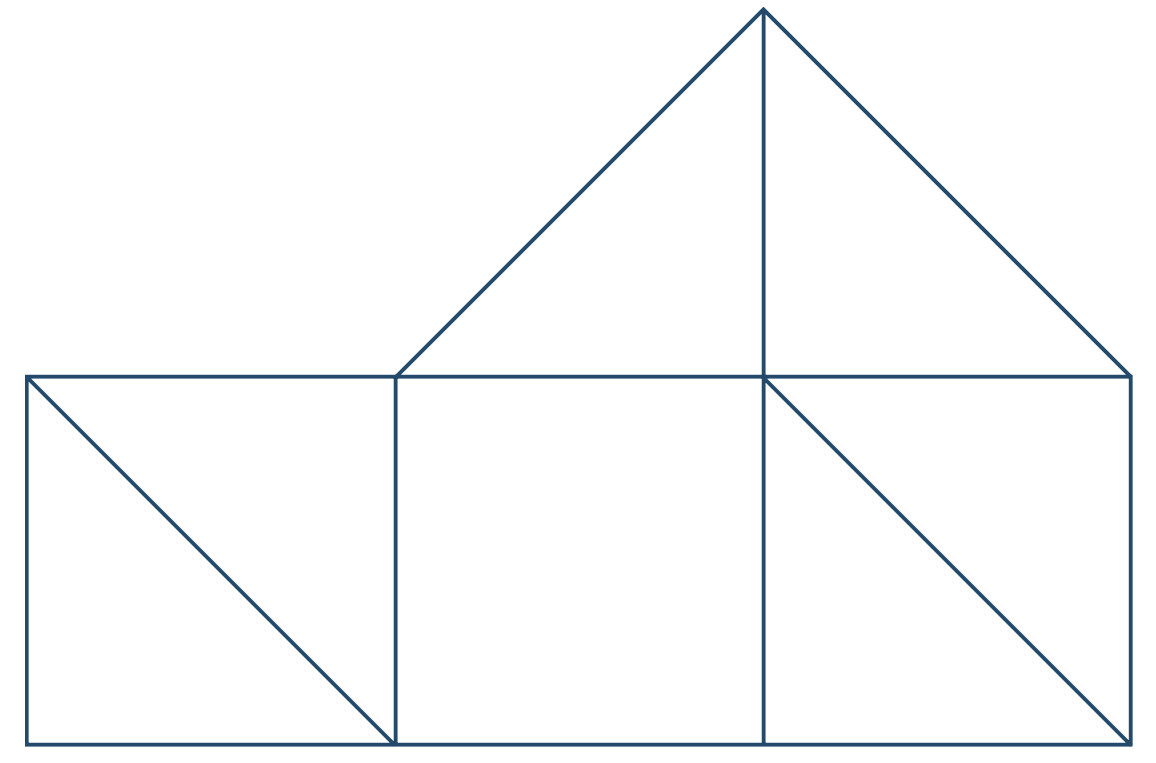
\includegraphics[width=0.5\textwidth]{figures/nodes.png}
\end{exercise}

\ifshowsolutions
\begin{solution}
Es gibt $n = 9$ Knoten, die den Verzweigungspunkten entsprechen.

Es gibt $b = 15$ Zweige, die den einzelnen Segmenten entsprechen, die zwei Knoten verbinden.

Insgesamt gibt es $l = 15$ geometrische Schleifen, d.,h. geschlossene Pfade. Aber nur $m = b - n + 1 = 7$ dieser geschlossenen Pfade sind unabhängige Schleifen. Man könnte die $7$ Maschen (die kleinsten möglichen Schleifen, die keine andere Schleife einschließen) für eine elektrische Netzwerkanalyse wählen, aber auch andere Kombinationen sind möglich.
\end{solution}
\fi

% ----- Exercise 2 -----
\begin{exercise}[KCL]
Bestimme  $i_1$, $i_2$ und $i_3$.

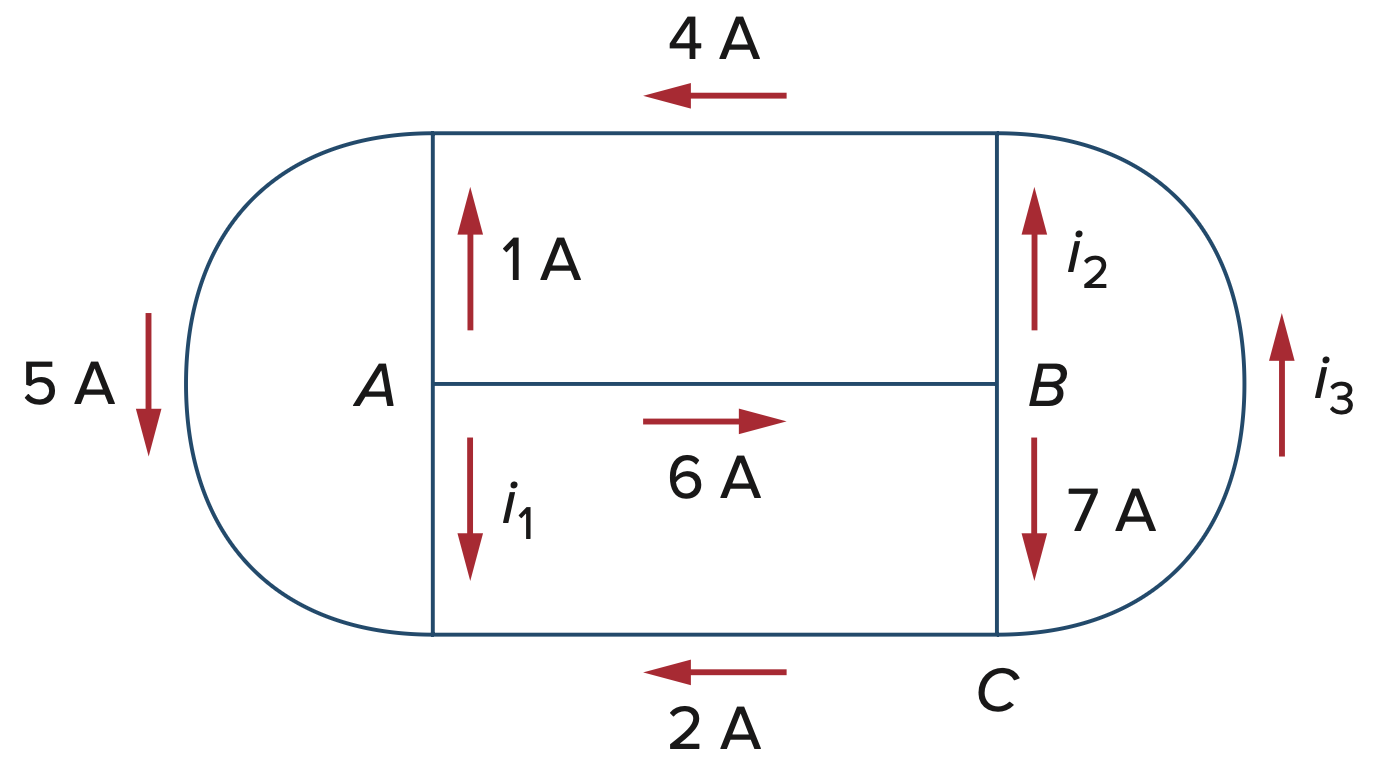
\includegraphics[width=0.7\textwidth]{figures/kcl.png}
\end{exercise}

\ifshowsolutions
\begin{solution}
Knoten A:
\[
-1\, \mathrm{A} - 6\, \mathrm{A} - i_1 = 0
\]
\[
\Rightarrow i_1 = -1\, \mathrm{A} - 6\, \mathrm{A} = -7\, \mathrm{A}
\]

Knoten B:
\[
6\, \mathrm{A} - 7\, \mathrm{A} - i_2 = 0
\]
\[
\Rightarrow i_2 = 6\, \mathrm{A} - 7\, \mathrm{A} = -1\, \mathrm{A}
\]

Knoten C:
\[
7\, \mathrm{A} - 2\, \mathrm{A} - i_3 = 0
\]
\[
\Rightarrow i_3 =  7\, \mathrm{A} - 2\, \mathrm{A}= 5\, \mathrm{A}
\]

... andere Knoten:
\[
i_2 + i_3 - 4\, \mathrm{A} = 0
\]
\[
\Rightarrow i_2 = 4\, \mathrm{A} - i_3 = -1\, \mathrm{A}
\]
\end{solution}
\fi

% ----- Exercise 3 -----
\begin{exercise}[KVL]
Berechne  $V_1$ und $V_2$.

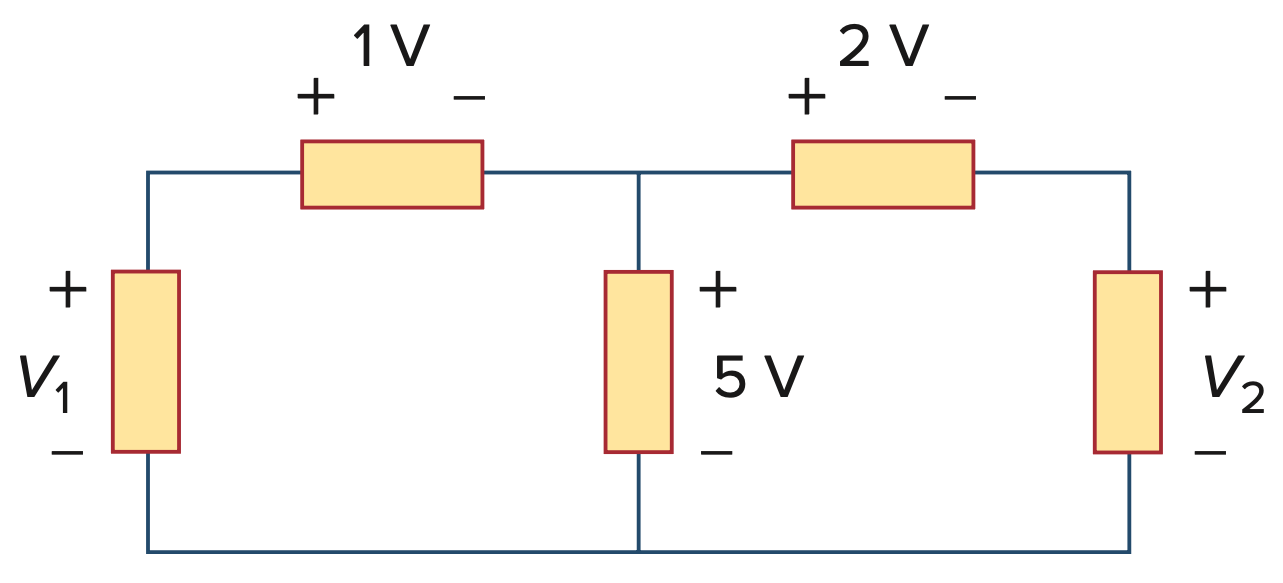
\includegraphics[width=0.7\textwidth]{figures/kvl.png}
\end{exercise}

\ifshowsolutions
\begin{solution}
\[
1\, \mathrm{V} + 5\, \mathrm{V} - V_1 = 0
\]
\[
\Rightarrow V_1 = 1\, \mathrm{V} + 5\, \mathrm{V} = 6\, \mathrm{V}
\]

\[
2\, \mathrm{V} + V_2 - 5\, \mathrm{V}= 0
\]
\[
\Rightarrow V_2 =  5\, \mathrm{V} - 2\, \mathrm{V}= 3\, \mathrm{V}
\]
\end{solution}
\fi

% ----- Exercise 4 -----
\begin{exercise}[Reihen- und Parallelschaltung von Widerständen]
Berechne $I_0$.

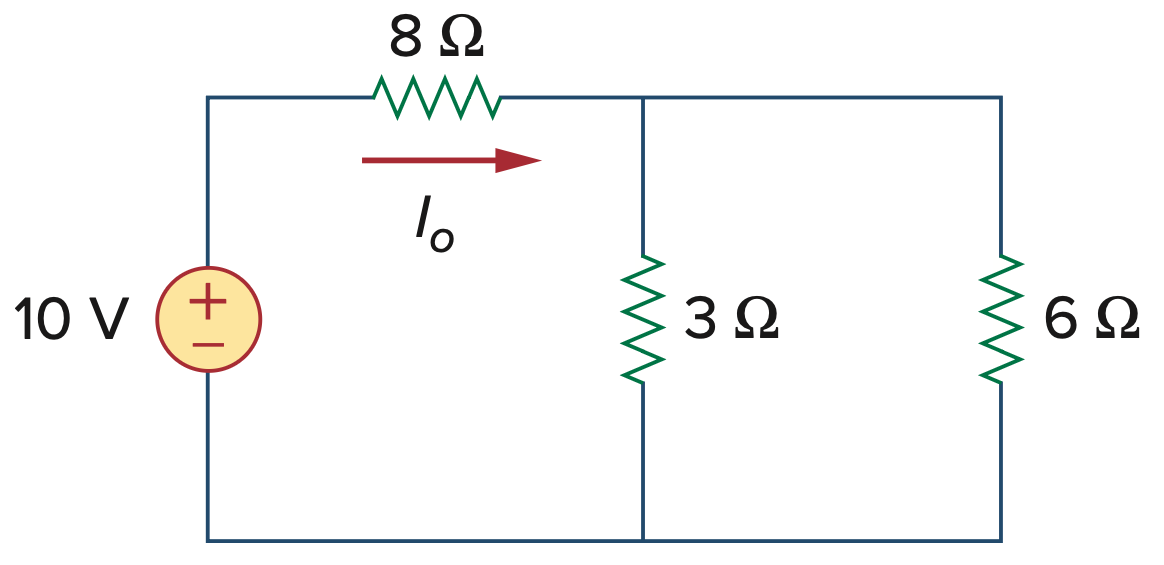
\includegraphics[width=0.7\textwidth]{figures/series_parallel.png}
\end{exercise}

\ifshowsolutions
\begin{solution}
Zunächst berechnen wir den Ersatzwiderstand der beiden parallelen Widerstände mit $3\, \Omega$ und $6\, \Omega$, dann addieren wir den Reihenwiderstand mit $8\, \Omega$ hinzu:

\[
R = \frac{3\, \Omega \cdot 6\, \Omega}{3\, \Omega + 6\, \Omega} + 8\, \Omega= 10\, \Omega
\]

Schließlich können wir mittels des Ohmschen Gesetzes die Stromstärke \(I_0\) brerechnen:

\[
I_o = \frac{10\, \mathrm{V}}{10\, \Omega} = 1\, \mathrm{A}
\]
\end{solution}
\fi

% ----- Exercise 5 -----
\begin{exercise}[Reihen- oder Parallelschaltung]
Drei Glühbirnen sind in Reihe an eine $120\, \mathrm{V}$-Quelle angeschlossen, wie unten gezeigt. Bestimme den Strom $I$ durch jede der Glühbirnen. Jede Glühbirne ist für $120\, \mathrm{V}$ ausgelegt. Wie viel Leistung nimmt jede Glühbirne auf? Erzeugen sie viel Licht?

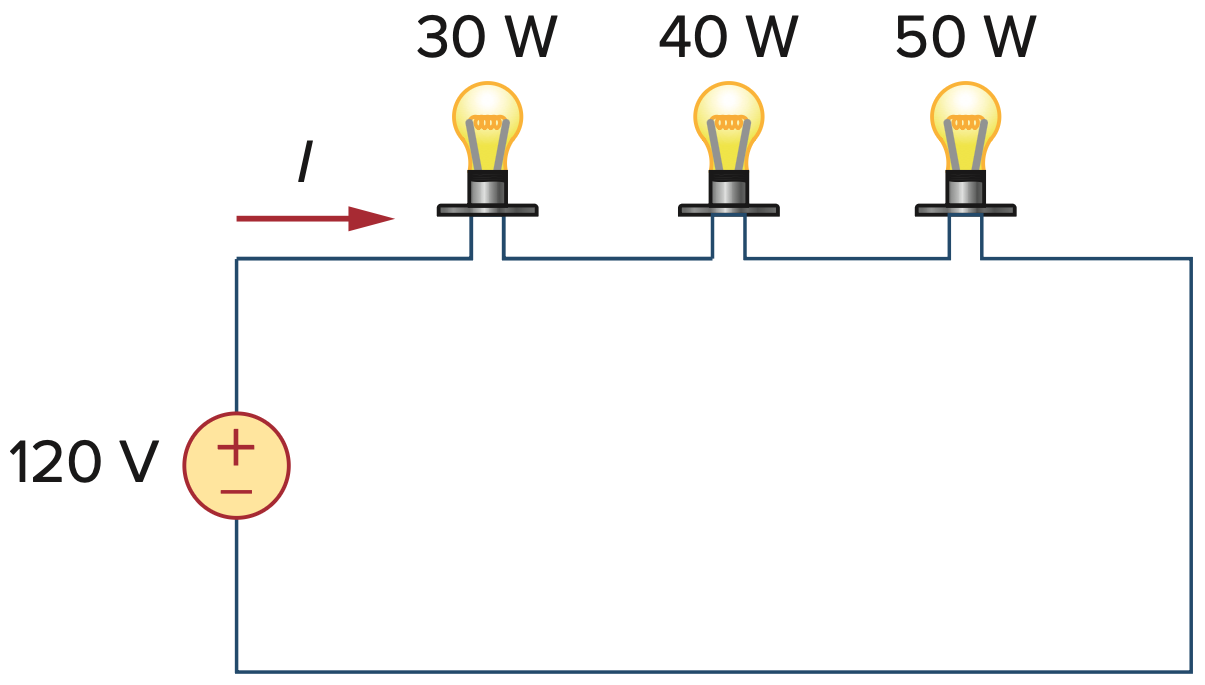
\includegraphics[width=0.7\textwidth]{figures/light_bulbs.png}
\end{exercise}

\ifshowsolutions
\begin{solution}
Zunächst berechnen wir die Widerstände jeder Glühbirne anhand ihrer Nennleistung und Spannung:
\[
R = \frac{V^2}{P}
\]

\[
R_{30\, \mathrm{W}} = \frac{(120\, \mathrm{V})^2}{30\, \mathrm{W}} = 480\, \Omega
\]

\[
R_{40\, \mathrm{W}} = \frac{(120\, \mathrm{V})^2}{40\, \mathrm{W}} = 360\, \Omega
\]

\[
R_{50\, \mathrm{W}} = \frac{(120\, \mathrm{V})^2}{50\, \mathrm{W}} = 288\, \Omega
\]

Dann berechnen wir den Ersatzwiderstand der drei in Reihe geschalteten Glühbirnen:
\[
R = 480\, \Omega + 360\, \Omega + 288\, \Omega = 1128\, \Omega
\]

Nun können wir die Stromstärke \(I\) mittels des Ohmschen Gesetzes berechnen:
\[
I = \frac{120\, \mathrm{V}}{1128\, \Omega} = 0.1063\, \mathrm{A}
\]  

Schließlich können wir die von jeder Glühbirne aufgenommene Leistung berechnen:
\[
P = I^2 \cdot R
\]

\[
P_{30\, \mathrm{W}} = (0.1063\, \mathrm{A})^2 \cdot 480\, \Omega = 5.432\, \mathrm{W}
\]

\[
P_{40\, \mathrm{W}} = (0.1063\, \mathrm{A})^2 \cdot 360\, \Omega = 4.074\, \mathrm{W}
\]

\[
P_{50\, \mathrm{W}} = (0.1063\, \mathrm{A})^2 \cdot 288\, \Omega = 3.259\, \mathrm{W}
\]

Offensichtlich liegen diese Werte weit unter den Nennleistungen jeder Glühbirne, sodass wir von keiner von ihnen viel Licht erwarten würden. Um richtig zu funktionieren, müssen sie parallel geschaltet werden.
\end{solution}
\fi

% ----- Exercise 6 -----
\begin{exercise}[Ersatzwiderstand]
Bestimme den Ersatzwiderstand $R_{ab}$ an den Klemmen.

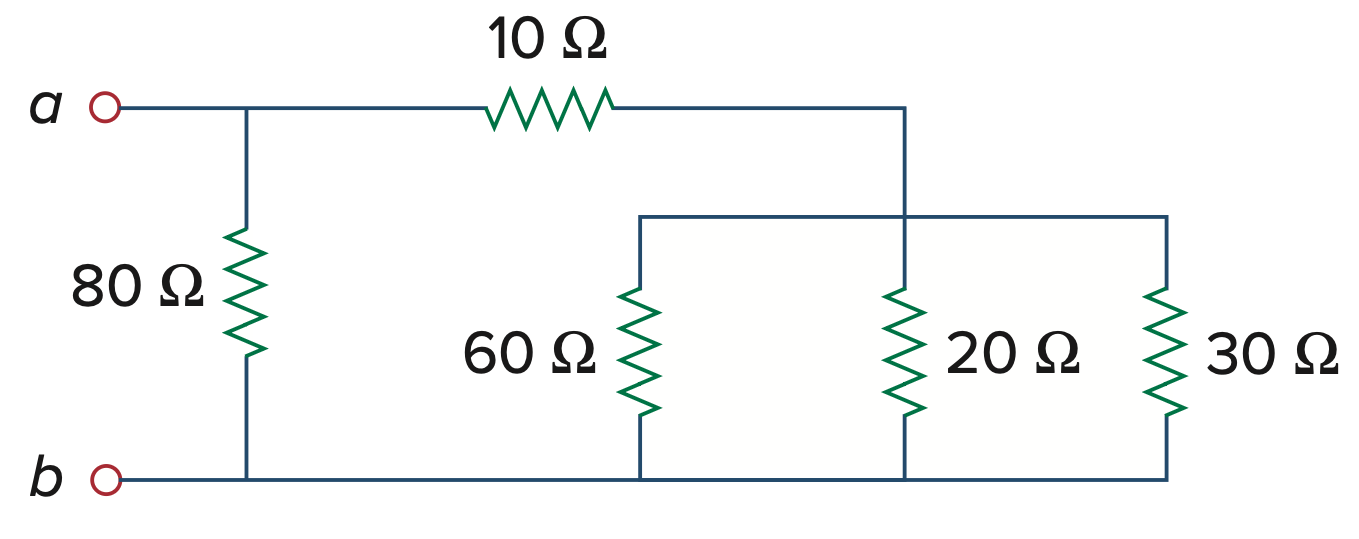
\includegraphics[width=0.7\textwidth]{figures/equivalent_R_1.png}
\end{exercise}

\ifshowsolutions
\begin{solution}
Zunächst berechnen wir den Ersatzwiderstand der parallelen Widerstände mit $60\, \Omega$, $20\, \Omega$ und $30\, \Omega$:
\[
R_p = \frac{1}{\frac{1}{60\, \Omega} + \frac{1}{20\, \Omega} + \frac{1}{30\, \Omega}} = 10\, \Omega
\]

Dann kombinieren wir diesen mit dem Reihenwiderstand von $10\, \Omega$:
\[
R_{ab} = 10\, \Omega + 10\, \Omega = 20\, \Omega
\]

Und schließlich kombinieren wir mit dem parallelen Widerstand von $80\, \Omega$:
\[
R_{ab} = \frac{1}{\frac{1}{20\, \Omega} + \frac{1}{80\, \Omega}} = 16\, \Omega
\]
\end{solution}
\fi

% ----- Exercise 7 -----
\begin{exercise}[Stromteiler]
Bestimme $i_1$ bis $i_5$.

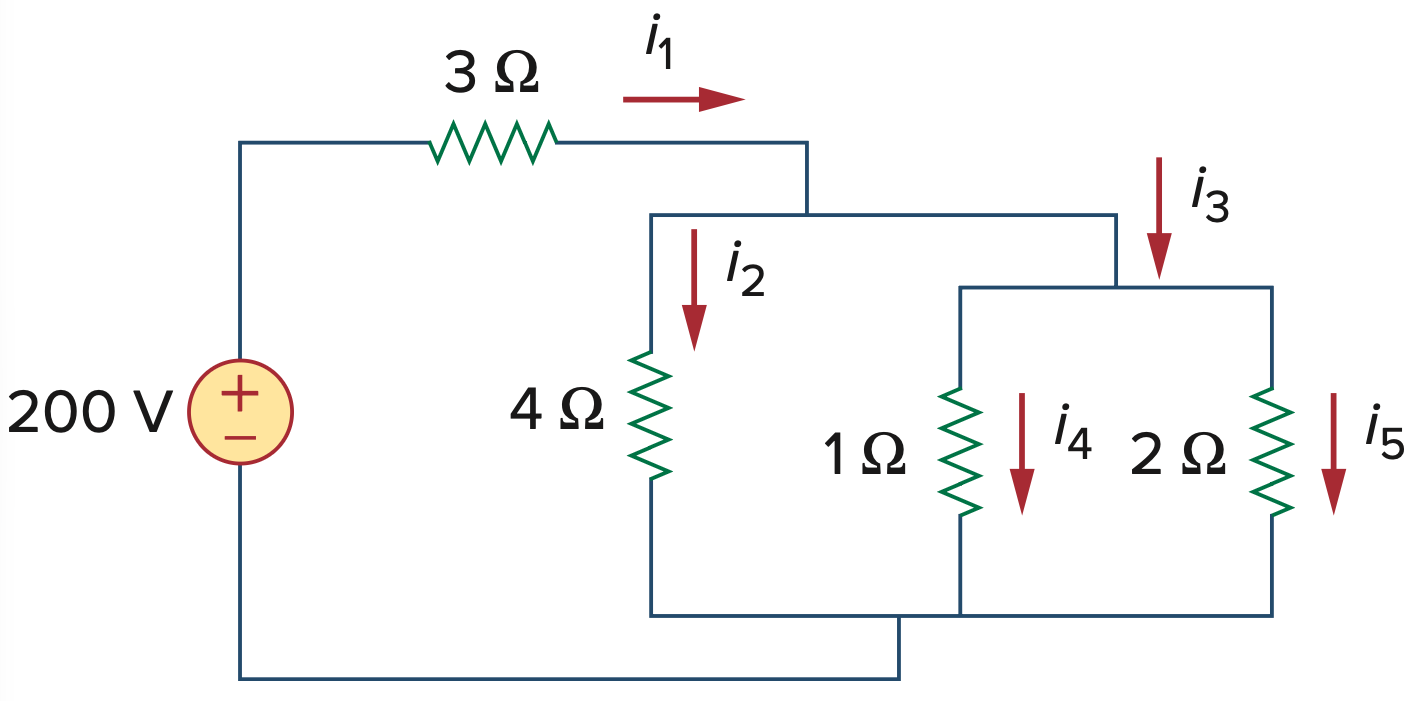
\includegraphics[width=0.7\textwidth]{figures/current_divider.png}
\end{exercise}

\ifshowsolutions
\begin{solution}
Zunächst berechnen wir den Ersatzwiderstand der parallelen Widerstände mit $1\, \Omega$ und $2\, \Omega$ und nennen ihn \(R_3\):

\[
R_3 = \frac{1\, \Omega \cdot 2\, \Omega}{1\, \Omega + 2\, \Omega} = \frac{2}{3}\, \Omega
\]

Dann berechnen wir den Gesamtwiderstand \(R\) aus dem $4\, \Omega$ Widerstand parallel zu \(R_3\) und dem $3\, \Omega$ Widerstand in Serie:

\[
R = 3\, \Omega + \frac{4\, \Omega \cdot \frac{2}{3}\, \Omega}{4\, \Omega + \frac{2}{3}\, \Omega} = \frac{25}{7}\, \Omega
\]

Unter Zuhilfenahme des Ohmschen Gesetzes können wir den Gesamtstrom \(i_1\) berechnen:

\[
i_1 = \frac{200\, \mathrm{V}}{\frac{25}{7}\, \Omega} = 56\, \mathrm{A}
\]

Nun können wir \(i_2\) mittels Stromteilung berechnen:

\[
i_2 = i_1 \cdot \frac{R_3}{R_2 + R_3} = 56\, \mathrm{A} \cdot \frac{\frac{2}{3}\, \Omega}{4\, \Omega + \frac{2}{3}\, \Omega} = 8\, \mathrm{A}
\]

KCL liefert uns \(i_3\):

\[
i_3 = i_1 - i_2 = 56\, \mathrm{A} - 8\, \mathrm{A} = 48\, \mathrm{A}
\]

Wiederum können wir \(i_4\) mittels Stromteilung berechnen:

\[
i_4 = i_3 \cdot \frac{R_5}{R_4 + R_5} = 48\, \mathrm{A} \cdot \frac{2\, \Omega}{1\, \Omega + 2\, \Omega} = 32\, \mathrm{A}
\]

Und schließlich liefert uns KCL \(i_5\):

\[
i_5 = i_3 - i_4 = 48\, \mathrm{A} - 32\, \mathrm{A} = 16\, \mathrm{A}
\]
\end{solution}
\fi

% ----- Exercise 8 -----
\begin{exercise}[Knotenverbindung]
Berechne $I_o$ und $V_o$.

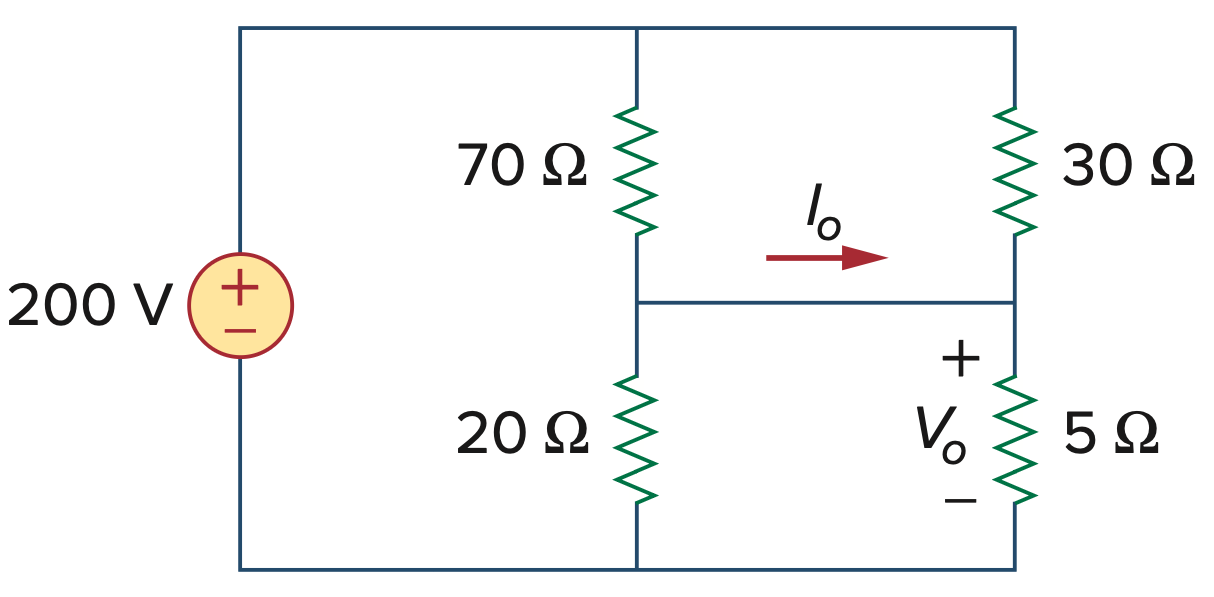
\includegraphics[width=0.7\textwidth]{figures/node_connection.png}
\end{exercise}

\ifshowsolutions
\begin{solution}
Ein Knoten ist ein Punkt, an dem zwei oder mehr Schaltungselemente verbunden sind (elektrisch derselbe Punkt). Ein Zweig ist ein Pfad, der zwei Knoten verbindet und ein Schaltungselement (Widerstand, Quelle usw.) enthält.

Hier gibt es drei Hauptknoten:
\begin{itemize}
  \item Oberer Knoten: verbunden mit der $+200\, \mathrm{V}$-Quelle, oberhalb der $70\, \Omega$ und $30\, \Omega$ Widerstände.
  \item Unterer Knoten: $0\, \mathrm{V}$ Referenz.
  \item Mittlerer Knoten: Verbindung zweier Zweige. Links der Zweig aus den Widerständen von $70\, \Omega$ und $20\, \Omega$. And rechts der Zweig aus den Widerständen von $30\, \Omega$ und $5\, \Omega$.
\end{itemize}

Der mittlere horizontale Draht (mit \(I_o\)) ist Teil des mittleren Knotens, aber da es einen Potentialunterschied zwischen dem linken und rechten Teil dieses Knotens gibt, bevor er verbunden wird, fließt Strom durch diese Verbindung — daher analysieren wir \(I_o\) so, als ob es sich um einen Zweigstrom handelt.

Da die Ausgangsspannung \(V_o\) die Spannung über dem $5\, \Omega$ Widerstand ist, entspricht die Ausgangsspannung der Spannung des mittleren Knotens.

\[
\text{Ströme vom oberen zum mittleren Knoten:}
\]
\[
I_{70} = \frac{200\, \mathrm{V} - V_o}{70\, \Omega}, \qquad I_{30} = \frac{200\, \mathrm{V} - V_o}{30\, \Omega}
\]

\[
\text{Ströme vom mittleren zum unteren Knoten:}
\]
\[
I_{20} = \frac{V_o}{20\, \Omega}, \qquad I_{5} = \frac{V_o}{5\, \Omega}
\]

Anwendung von KCL am mittleren Knoten:
\[
\frac{200\, \mathrm{V} - V_o}{70\, \Omega} + \frac{200\, \mathrm{V} - V_o}{30\, \Omega} = \frac{V_o}{20\, \Omega} + \frac{V_o}{5\, \Omega}
\]

Vereinfachen:
\[
\frac{200\, \mathrm{V} - V_o}{21\, \Omega} = \frac{V_o}{4\, \Omega}
\]

\[
\Rightarrow 800\, \mathrm{V} - 4 \cdot V_o = 21 \cdot V_o
\]

\[
\Rightarrow \boxed{V_o = 32~\text{V}}
\]

Jetzt verwenden wir KCL, um den Strom \(I_o\) (definiert nach rechts) zu berechnen:

\[
I_o = I_{70} - I_{20} = \frac{200\, \mathrm{V} - 32\, \mathrm{V}}{70\, \Omega} - \frac{32\, \mathrm{V}}{20\, \Omega} =\boxed{0.8\, \mathrm{A}}
\]
\end{solution}
\fi

% ----- Exercise 9 -----
\begin{exercise}[Schaltungsberechnung]
Berechne den Ersatzwiderstand an den Klemmen.

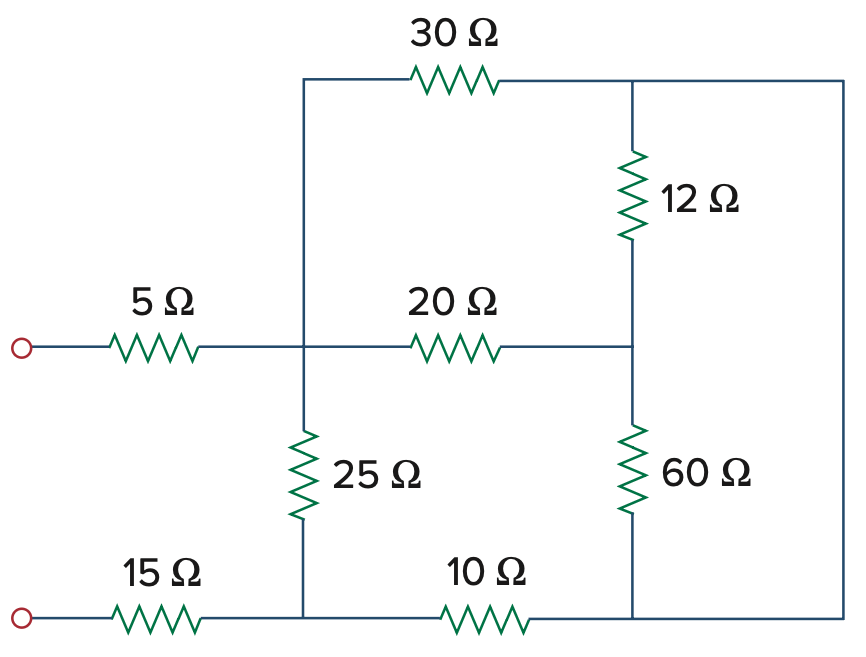
\includegraphics[width=0.7\textwidth]{figures/equivalent_R_2.png}
\end{exercise}

\ifshowsolutions
\begin{solution}
1. Kombiniere die vertikalen Widerstände auf der rechten Seite:
\[
12\, \Omega \parallel 60\, \Omega = \frac{12\, \Omega \cdot 60\, \Omega}{12\, \Omega + 60\, \Omega} = 10\, \Omega
\]

2. Reihenkombination mit dem $20\, \Omega$-Widerstand:
\[
20\, \Omega + 10\, \Omega = 30\, \Omega
\]

3. Parallelkombination mit dem anderen $30\, \Omega$-Widerstand:
\[
30\, \Omega \parallel 30\, \Omega = \frac{30\, \Omega \cdot 30\, \Omega}{30\, \Omega + 30\, \Omega} = 15\, \Omega
\]

Nach diesen drei Schritten reduziert sich die Schaltung zu einem Dreieck ($\Delta$):

\begin{center}
\begin{circuitikz}[american]
    \draw
    (0,0) node[anchor=east]{}
    to[R=$15\,\Omega$, o-*] (2,0)
    to[short] (3,0)
    to[R=$10\,\Omega$] (5,0)
    node[circle,draw,fill=white,inner sep=1pt,label=below:$N_3$]{};

    \node[circle,draw,fill=black,inner sep=1pt,label=above:$N_1$] (N1) at (2,4) {};
    \node[circle,draw,fill=black,inner sep=1pt,label=below:$N_2$] (N2) at (2,0) {};

    \draw
    (0,4) node[anchor=east]{}
    to[R=$5\,\Omega$, o-*] (2,4)
    to[R=$25\,\Omega$] (2,0)
    (2,4) to[R=$15\,\Omega$] (5,0);
\end{circuitikz}
\end{center}

4. Konvertiere das $\Delta$-Netzwerk in äquivalente Y-Widerstände:
\[
R_1 = \frac{R_b R_c}{R_a + R_b + R_c} = \frac{15\, \Omega \cdot 25\, \Omega}{50\, \Omega} = 7.5\, \Omega
\]
\[
R_2 = \frac{R_a R_c}{R_a + R_b + R_c} = \frac{10\, \Omega \cdot 25\, \Omega}{50\, \Omega} = 5\, \Omega
\]
\[
R_3 = \frac{R_a R_b}{R_a + R_b + R_c} = \frac{10\, \Omega \cdot 15\, \Omega}{50\, \Omega} = 3\, \Omega
\]

\begin{center}
\begin{circuitikz}[american]
    % Nodes
    \node[] (A) at (0,4) {};
    \node[] (B) at (0,0) {};
    \node[circle,draw,fill=white,inner sep=1pt,label=above:$N_1$] (N1) at (2,3) {};
    \node[circle,draw,fill=white,inner sep=1pt,label=below:$N_2$] (N2) at (2,1) {};
    \node[circle,draw,fill=white,inner sep=1pt,label=right:$N_3$] (N3) at (5,2) {};
    \node[circle,draw,fill=white,inner sep=1pt] (O) at (3.5,2) {}; % star center

    % External connections
    \draw (A) to[R=$5\,\Omega$, o-*] (N1);
    \draw (B) to[R=$15\,\Omega$, o-*] (N2);

    % Star (Y) arms
    \draw (O) to[R=$7.5\,\Omega$] (N1);
    \draw (O) to[R=$5\,\Omega$] (N2);
    \draw (O) to[R=$3\,\Omega$] (N3);

\end{circuitikz}
\end{center}

Der Zweig mit dem \( 3\, \Omega \)-Widerstand verbindet sich mit einem losen Knoten \( N_3 \), sodass kein Strom fließt und dieser ignoriert werden kann.
\[
\Rightarrow R_{eq} = 5\, \Omega + 7.5\, \Omega + 5\, \Omega + 15\, \Omega = 32.5\, \Omega
\]

Alternative für 4. ohne $\Delta$-Y Transformation:

Da \( N_3 \) ein trivialer Knoten ist (nur ein Eingang und ein gleicher Ausgang), kann man einfach den Serienwiderstand der \( 15\, \Omega \) und \( 10\, \Omega \) Widerstände berechnen, ihn dann parallel mit dem \( 25\, \Omega \) Widerstand kombinieren und schließlich die Serienwiderstände mit \( 5\, \Omega \) und \( 15\, \Omega \) addieren.
\end{solution}
\fi

\end{document}